\documentclass{article}
\usepackage{graphicx}
\usepackage[margin=1.5cm]{geometry}
\usepackage{amsmath}

\begin{document}
\small
\title{Warm Up: Work and Energy}
\author{Prof. Jordan C. Hanson}

\maketitle

\section{Memory Bank}

\begin{itemize}
\item $W = \vec{F} \cdot \Delta \vec{x}$ ... Definition of work
\item $\vec{a} \cdot \vec{b} = a_x b_x + a_y b_y$ ... The dot-product of $\vec{a}$ and $\vec{b}$. The components of $\vec{a}$ and $\vec{b}$ are $a_x$ and $a_y$, and $b_x$ and $b_y$, respectively.
\item $\vec{a} \cdot \vec{b} = |\vec{a}| |\vec{b}| \cos\theta$ ... The dot-product of $\vec{a}$ and $\vec{b}$.  The magnitude of $\vec{a}$ is $|\vec{a}|$, and the magnitude of $\vec{b}$ is $|\vec{b}|$.
\item $KE = \frac{1}{2}m v^2$ ... Definition of Kinetic Energy
\item $W = KE_f - KE_i$ ... Work-energy theorem.
\item $\int k ~ dx = kx + C$ ... The \textit{integral} of a constant function, $f(x) = k$, where $C$ is some constant.
\item $\int k x ~ dx = \frac{1}{2}k x^2 + C$ ... The \textit{integral} of a linear function, $f(x) = kx$, where $C$ is some constant.
\end{itemize}

\begin{figure}
\centering
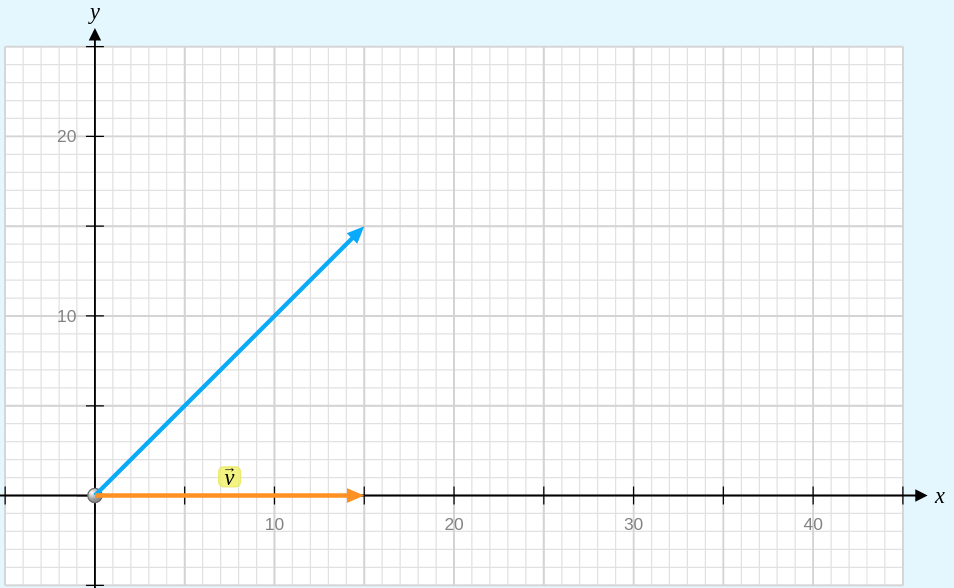
\includegraphics[width=0.3\textwidth,trim=0cm 0cm 3cm 0cm,clip=true]{figures/vec1.png}
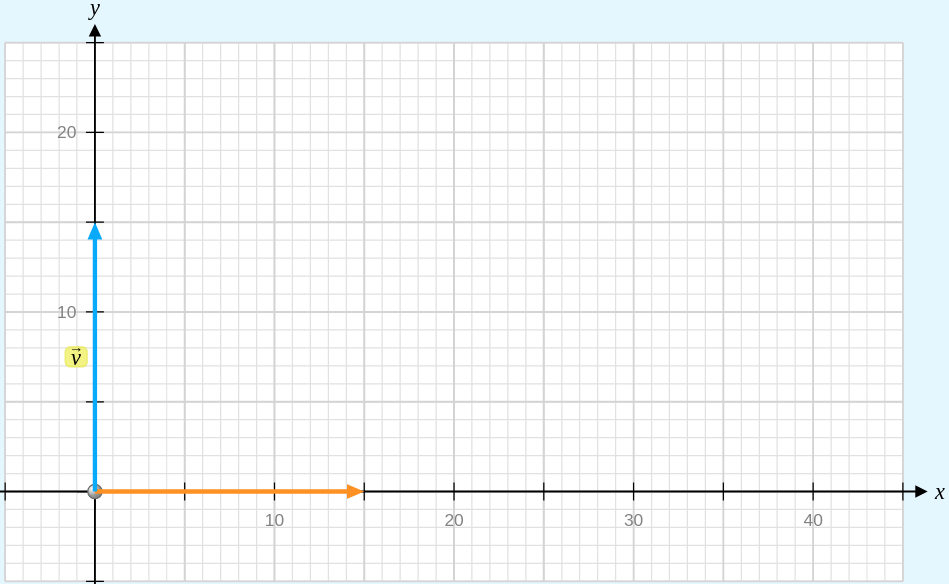
\includegraphics[width=0.3\textwidth,trim=0cm 0cm 3cm 0cm,clip=true]{figures/vec2.png}
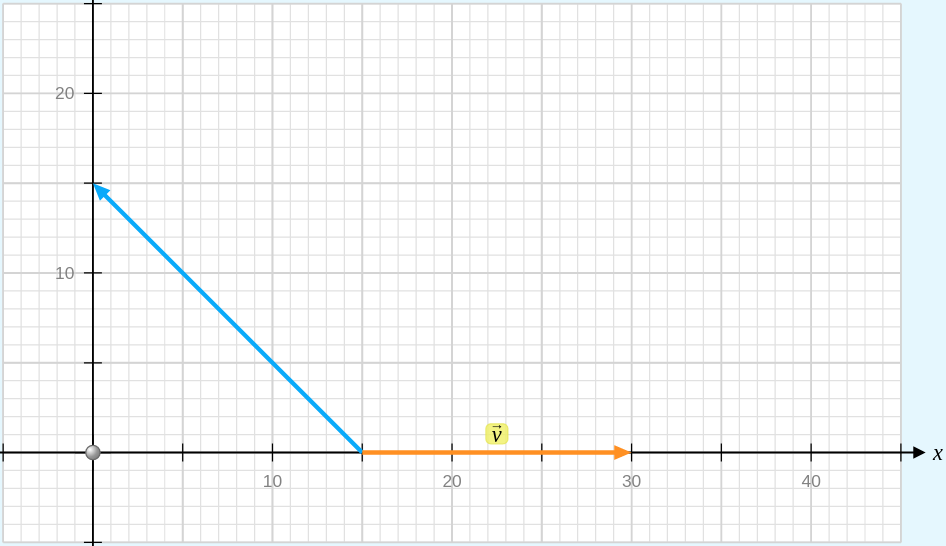
\includegraphics[width=0.3\textwidth,trim=0cm 0cm 3cm 0cm,clip=true]{figures/vec3.png}
\caption{\label{fig:1} (Left) Two vectors separated by 45 degrees. (Middle) Two vectors separated by 90 degrees. (Right) Two vectors separated by 135 degrees.}
\end{figure}

\section{Work and Energy}

\begin{enumerate}
\item In Fig. \ref{fig:1} below, assume that the upper vector represents force and the lower vector represents displacement. (a) Which scenario (left, middle, or right) corresponds to the maximum amount of work done on the system? (b) In Fig. \ref{fig:1} (left), let $\vec{F} = 15\hat{i} + 15\hat{j}$ N and $\Delta \vec{x} = 15\hat{i}$ meters.  What is the work done? (c) For Fig. \ref{fig:1} (middle), if $\Delta \vec{x} = 15\hat{i}$ meters, and $W = 0$, what is $\vec{F}$? (d) What is the ratio of the work in Fig. \ref{fig:1} (left) to the work in Fig. \ref{fig:1} (right)? \\ \vspace{2cm}
\item Suppose the system in Fig. \ref{fig:1} (left) has a mass of 10 kg, and the work done is 100 J through a displacement of 2 meters.  (a) What is the magnitude of the force? (b) What is the force as a vector? (c) If the total work done is 100 J, what is the final velocity of the system?
\end{enumerate}

\end{document}
